\documentclass[preprint,12pt]{elsarticle}
\usepackage[utf8]{inputenc}
\usepackage[numbers]{natbib}
\bibliographystyle{abbrvnat}
\usepackage{graphicx}

%% Use the option review to obtain double line spacing
%% \documentclass[preprint,review,12pt]{elsarticle}

%% Use the options 1p,twocolumn; 3p; 3p,twocolumn; 5p; or 5p,twocolumn
%% for a journal layout:
%% \documentclass[final,1p,times]{elsarticle}
%% \documentclass[final,1p,times,twocolumn]{elsarticle}
%% \documentclass[final,3p,times]{elsarticle}
%% \documentclass[final,3p,times,twocolumn]{elsarticle}
%% \documentclass[final,5p,times]{elsarticle}
%% \documentclass[final,5p,times,twocolumn]{elsarticle}

%% if you use PostScript figures in your article
%% use the graphics package for simple commands
%% \usepackage{graphics}
%% or use the graphicx package for more complicated commands
%% \usepackage{graphicx}
%% or use the epsfig package if you prefer to use the old commands
%% \usepackage{epsfig}

%% The amssymb package provides various useful mathematical symbols
\usepackage{amssymb}
%% The amsthm package provides extended theorem environments
%% \usepackage{amsthm}

%% The lineno packages adds line numbers. Start line numbering with
%% \begin{linenumbers}, end it with \end{linenumbers}. Or switch it on
%% for the whole article with \linenumbers after \end{frontmatter}.
%%\usepackage{lineno}

%% natbib.sty is loaded by default. However, natbib options can be
%% provided with \biboptions{...} command. Following options are
%% valid:

%%   round  -  round parentheses are used (default)
%%   square -  square brackets are used   [option]
%%   curly  -  curly braces are used      {option}
%%   angle  -  angle brackets are used    <option>
%%   semicolon  -  multiple citations separated by semi-colon
%%   colon  - same as semicolon, an earlier confusion
%%   comma  -  separated by comma
%%   numbers-  selects numerical citations
%%   super  -  numerical citations as superscripts
%%   sort   -  sorts multiple citations according to order in ref. list
%%   sort&compress   -  like sort, but also compresses numerical citations
%%   compress - compresses without sorting
%%
%% \biboptions{comma,round}

% \biboptions{}
\usepackage{mathtools}

\usepackage[subpreambles=true]{standalone}


\begin{document}

\begin{frontmatter}

%% Title, authors and addresses

%% use the tnoteref command within \title for footnotes;
%% use the tnotetext command for the associated footnote;
%% use the fnref command within \author or \address for footnotes;
%% use the fntext command for the associated footnote;
%% use the corref command within \author for corresponding author footnotes;
%% use the cortext command for the associated footnote;
%% use the ead command for the email address,
%% and the form \ead[url] for the home page:
%%
%% \title{Title\tnoteref{label1}}
%% \tnotetext[label1]{}
%% \author{Name\corref{cor1}\fnref{label2}}
%% \ead{email address}
%% \ead[url]{home page}
%% \fntext[label2]{}
%% \cortext[cor1]{}
%% \address{Address\fnref{label3}}
%% \fntext[label3]{}

\title{Approche hybride pour résoudre le problème du Bin Packing}

%% use optional labels to link authors explicitly to addresses:
%% \author[label1,label2]{<author name>}
%% \address[label1]{<address>}
%% \address[label2]{<address>}

\author{BACHI Yasmine, MIHOUBI LamiaZohra , MOUSSAOUI Meroua, NOUALI Sarah, SAADI Khaoula}

\address{Ecole nationale Supérieure d'Informatique -ESI-Alger}
\date{26 juin 2020}
\begin{abstract}
%% Text of abstract
L’objectif du problème du bin packing (BPP) est de trouver le nombre minimal de boîtes nécessaire pour ranger un ensemble de n objets ayant des tailles connues, en respectant la capacité de chaque boîte. Ce problème est parmis les problèmes NP-difficile. Dans cet article, on propose un algorithme génétique  hybride utilisant le recuit simulé. Les résultats expérimentaux   ont montré l’efficacité de notre hybridation dans l’amélioration de la qualité de solution de l’algorithme génétique pour les classes 1 et 2 du benchmark Scholl. \end{abstract}

\begin{keyword}
%% keywords here, in the form: keyword \sep keyword
Bin packing \sep hybridation \sep AG \sep recuit simulé 
%% MSC codes here, in the form: \MSC code \sep code
%% or \MSC[2008] code \sep code (2000 is the default)

\end{keyword}

\end{frontmatter}

%%
%% Start line numbering here if you want
%%
%%\linenumbers

%% main text
\section{Introduction}
\label{S:1}

Le problème du bin packing à une dimension (BPP) est défini comme suit, étant donné un nombre illimité de boîtes avec une capacité fixe C, et un ensemble de n objets, chacun ayant un poid spécifique 0<wi<C, on cherche à ranger les n objets dans un nombre minimal de boîte, tout en respectant la capacité C. 


\subsection{Algorithme génétique (AG)}
L’algorithme génétique est une heuristique de recherche initialement proposée par Holland [1] qui imite le processus de sélection naturelle.Elle appartient à la plus grande classe d'algorithmes évolutionnaires (EA), qui génèrent des solutions en utilisant des techniques inspirées de l'évolution naturelle, telles que la mutation, la sélection et le croisement.

La figure suivante représente les étapes de fonctionnement de notre AG, avec la spécification des méthodes utilisées pour implémenter chaque étape. 

\begin{figure}[h]
    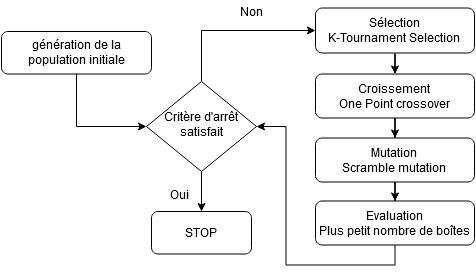
\includegraphics[width=\linewidth]{./figures/AG schema.png}
    \caption{Processus de AG }
    \label{fig:agschema}
\end{figure}
Les algorithmes génétiques sont connus par leur Rapidité et facilité d’utilisation. 
En effet, le AG est parmis les métaheuristiques les plus rapides, de plus, si la la représentation vectorielle de l'individu est correcte, nous pouvons trouver une solution sans un travail d'analyse approfondi. Par contre, cette métaheuristique ne trouve pas toujours l’optimum et peut se retrouver avec le problème d’optimum local. 

\subsection{Le Recuit Simulé (SA)}
Le recuit simulé est un algorithme de recherche locale initialement introduit par Kirkpatrick et al \cite{kirk} qui simule la fusion et le refroidissement dans le traitement des métaux. Le recuit simulé est généralement implémenté pour rechercher une solution optimale sur une petite zone, même s'il est parfois aussi performant que AG dans certains cas \cite{Alkhateeb}.
Cette métaheuristique sophistiquée empêche d'être piégé dans les minima locaux à l'aide d'un moteur de recherche aléatoire exprimé en termes de chaîne de Markov. Elle introduit des changements dans la solution pour améliorer la fonction objectif, mais conserve également des solutions qui, malgré les moins bonnes performances, répondent à certains critères. Mais l’un des inconvénients du recuit simulé est son temps d'exécution élevé. 

\subsection{Hybridation}
Pour surmonter les inconvénients  de GA et SA, plusieurs études proposent une hybridation entre les deux.
Junghans et Darde \cite{Junghans} comparent entre AG et AG hybride avec SA modifiée (MSA).
Le SA utilisé dans leur expérience a été modifié pour contrôler la réduction de la température.
Ils ont découvert que le GA-MSA hybride offre une fiabilité plus élevée que le AG.
Une autre recherche menée par Chen et Shahandashti dans \cite{Chen} qui compare également le GA, SA, un hybride de GA-SA et MSA, où ils ont constaté que le GA-SA hybride est plus performante que AG, SA et MSA. \\
Dans cet article, nous avons hybridé le GA-SA avec quatres scénarios, à savoir le AG-RS hybride,le AGH-RS , le AG-2RS et le AG-MIX, Le schéma hybride AG-RS consiste à obtenir la meilleure solution en AG et à l'utiliser comme population initiale en SA,
le AGH-RS utilise le même processus sauf que AG à été initialisé par plusieurs heuristiques.Le schema AG-2RS  consiste à inclure SA dans le AG après l’étape de mutation, et améliorer la solution de AG par le SA à nouveau. finalement le schéma AG-MIX utilise le même processus que AG-2RS en initialisant le AG par plusieurs heuristiques. 
D’autres schémas ont été implémenté et serons inclus dans la comparaison, on cite le WOA-RS  et le ILWOA-RS qui sont une hybridation de haut niveau des métaheuristiques WOA et ILWOA avec le recuit simulé.

 
 \subsection{Organisation du papier}
 On va tout d’abord définir le problème du bin packing, sa représentation mathématique, par la suite on présentera nos schémas hybrides proposés. Finalement, des résultats expérimentaux sont donnés et une comparaison des schémas hybrides est effectuée  dans [ num], suivi d’une conclusion.

\section{Formulation du problème}
\subsection{Défénition du problème}
Le problème du bin packing à une dimension (BPP) est défini comme suit, étant donné un nombre illimité de boîtes avec une capacité fixe C, et un ensemble de n objets, chacun ayant un poid spécifique 0<wi<C, on cherche à ranger les n objets dans un nombre minimal de boîte, tout en respectant la capacité C. 

\subsection{Formulation mathématique}
Etant donné \(m\) boites de capacité \(C\) et \(n\) articles de volume \(v_i\) chacun. \\
    Soient: 
    \[ x_{ij} =
        \begin{cases}
            1  & \quad \text{article } j \text{ rangé dans la boîte } i \\
            0  & \quad \text{sinon } 
        \end{cases}
    \]
    \[ y_i =
    \begin{cases}
        1  & \quad \text{boîte } i \text{ utilisée } \\
        0  & \quad \text{sinon } 
    \end{cases}
    \]

La formulation du problème donne ainsi le programme linéaire suivant
\[(PN)
    \begin{cases}
        Z(min) = \displaystyle\sum_{i=1}^{m} y_i \\
        \displaystyle\sum_{i=1}^{m} x_{ij}  = 1 \\
        \displaystyle\sum_{j=1}^{n} v_j x_{ij} \le C y_i \\
        y_i \in \{0,1\} \\
        x_{ij} \in \{0,1\} 
    \end{cases}
\]  
La première contrainte signifie qu’un article j ne peut être placé qu’en une seule boite
La deuxième fait qu’on ne dépasse pas la taille d’une boite lors du rangement

\section{L'approche hybride proposée}

\subsection{Encodage de la solution}
\subsection{L'hybridation AG-RS}
\medskip

\bibliography{Samples}


\begin{table}[h]
\centering
\begin{tabular}{l l l}
\hline
\textbf{Treatments} & \textbf{Response 1} & \textbf{Response 2}\\
\hline
Treatment 1 & 0.0003262 & 0.562 \\
Treatment 2 & 0.0015681 & 0.910 \\
Treatment 3 & 0.0009271 & 0.296 \\
\hline
\end{tabular}
\caption{Table caption}
\end{table}




\subsection{Subsection Two}

Donec eget ligula venenatis est posuere eleifend in sit amet diam. Vestibulum sollicitudin mauris ac augue blandit ultricies. Nulla facilisi. Etiam ut turpis nunc. Praesent leo orci, tincidunt vitae feugiat eu, feugiat a massa. Duis mauris ipsum, tempor vel condimentum nec, suscipit non mi. Fusce quis urna dictum felis posuere sagittis ac sit amet erat. In in ultrices lectus. Nulla vitae ipsum lectus, a gravida erat. Etiam quam nisl, blandit ut porta in, accumsan a nibh. Phasellus sodales euismod dolor sit amet elementum. Phasellus varius placerat erat, nec gravida libero pellentesque id. Fusce nisi ante, euismod nec cursus at, suscipit a enim. Nulla facilisi.

\begin{figure}[h]

\caption{Figure caption}
\end{figure}

Integer risus dui, condimentum et gravida vitae, adipiscing et enim. Aliquam erat volutpat. Pellentesque diam sapien, egestas eget gravida ut, tempor eu nulla. Vestibulum mollis pretium lacus eget venenatis. Fusce gravida nisl quis est molestie eu luctus ipsum pretium. Maecenas non eros lorem, vel adipiscing odio. Etiam dolor risus, mattis in pellentesque id, pellentesque eu nibh. Mauris nec ante at orci ultricies placerat ac non massa. Aenean imperdiet, ante eu sollicitudin vestibulum, dolor felis dapibus arcu, sit amet fermentum urna nibh sit amet mauris. Suspendisse adipiscing mollis dolor quis lobortis.

\begin{equation}
\label{eq:emc}
e = mc^2
\end{equation}

\section{The Second Section}
\label{S:2}

Reference to Section \ref{S:1}. Etiam congue sollicitudin diam non porttitor. Etiam turpis nulla, auctor a pretium non, luctus quis ipsum. Fusce pretium gravida libero non accumsan. Donec eget augue ut nulla placerat hendrerit ac ut mi. Phasellus euismod ornare mollis. Proin tempus fringilla ultricies. Donec pretium feugiat libero quis convallis. Nam interdum ante sed magna congue eu semper tellus sagittis. Curabitur eu augue elit.

Aenean eleifend purus et massa consequat facilisis. Etiam volutpat placerat dignissim. Ut nec nibh nulla. Aliquam erat volutpat. Nam at massa velit, eu malesuada augue. Maecenas sit amet nunc mauris. Maecenas eu ligula quis turpis molestie elementum nec at est. Sed adipiscing neque ac sapien viverra sit amet vestibulum arcu rhoncus.

Vivamus pharetra nibh in orci euismod congue. Pellentesque habitant morbi tristique senectus et netus et malesuada fames ac turpis egestas. Quisque lacus diam, congue vel laoreet id, iaculis eu sapien. In id risus ac leo pellentesque pellentesque et in dui. Etiam tincidunt quam ut ante vestibulum ultricies. Nam at rutrum lectus. Aenean non justo tortor, nec mattis justo. Aliquam erat volutpat. Nullam ac viverra augue. In tempus venenatis nibh quis semper. Maecenas ac nisl eu ligula dictum lobortis. Sed lacus ante, tempor eu dictum eu, accumsan in velit. Integer accumsan convallis porttitor. Maecenas pretium tincidunt metus sit amet gravida. Maecenas pretium blandit felis, ac interdum ante semper sed.

In auctor ultrices elit, vel feugiat ligula aliquam sed. Curabitur aliquam elit sed dui rhoncus consectetur. Cras elit ipsum, lobortis a tempor at, viverra vitae mi. Cras sed urna sed eros bibendum faucibus. Morbi vel leo orci, vel faucibus orci. Vivamus urna nisl, sodales vitae posuere in, tempus vel tellus. Donec magna est, luctus non commodo sit amet, placerat et enim.

%% The Appendices part is started with the command \appendix;
%% appendix sections are then done as normal sections
%% \appendix

%% \section{}
%% \label{}

%% References
%%
%% Following citation commands can be used in the body text:
%% Usage of \cite is as follows:
%%   \cite{key}          ==>>  [#]
%%   \cite[chap. 2]{key} ==>>  [#, chap. 2]
%%   \citet{key}         ==>>  Author [#]

%% References with bibTeX database:
%% Authors are advised to submit their bibtex database files. They are
%% requested to list a bibtex style file in the manuscript if they do
%% not want to use model1-num-names.bst.

%% References without bibTeX database:

% \begin{thebibliography}{00}

%% \bibitem must have the following form:
%%   \bibitem{key}...
%%

% \bibitem{}

% \end{thebibliography}

\end{document}

%%
%% End of file `elsarticle-template-1-num.tex'.
